% !TEX root = main.tex

\section{二元决策图}
$\cdot$为与,$+$为或,$\oplus$为异或。

布尔函数用真值表表示,如$f(x,y)\eqdef\overline{x+y}$。
\begin{center}
\begin{tabular}{cc|c}
$x$ & $y$ & $f(x,y)$\\\hline
$1$ & $1$ & $0$ \\
$1$ & $0$ & $1$ \\
$0$ & $1$ & $0$ \\
$0$ & $0$ & $1$
\end{tabular}
\end{center}

二元决策图(Binary Decision Diagram, BDD)
\begin{itemize}
	\item 非终端结点标号为布尔变量
	\item 终端结点(叶子)标号为0或1
	\item 每一个非终端结点有两条边,一条虚边(dashed)指向0,一条实边(solid)指向1
\end{itemize}

简化法则\footnote{图源来自Cornell ECE5775: \url{https://www.csl.cornell.edu/courses/ece5775/pdf/lecture05.pdf}}:
\begin{itemize}
	\item 合并等价叶子结点(只留0和1各一个)
	\begin{figure}[H]
	\centering
	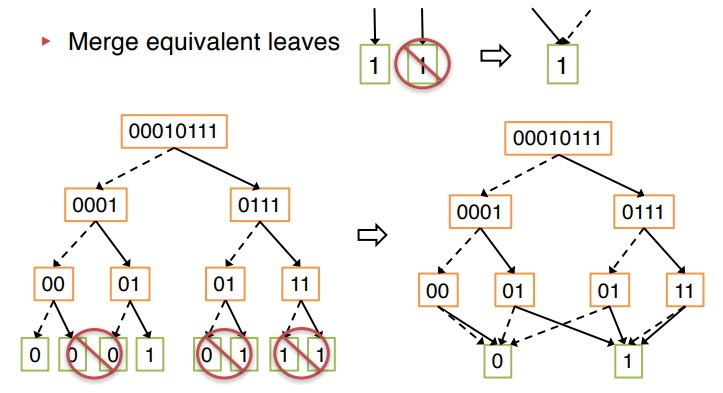
\includegraphics[width=0.8\linewidth]{fig/bdd_reduction1.jpg}
	\end{figure}
	\item 去除冗余测试(test)
	\begin{figure}[H]
	\centering
	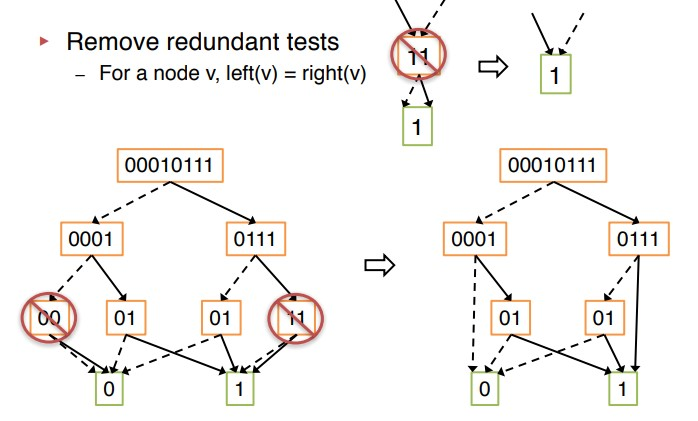
\includegraphics[width=0.8\linewidth]{fig/bdd_reduction2.jpg}
	\end{figure}
	\item 合并同构结点
	\begin{figure}[H]
	\centering
	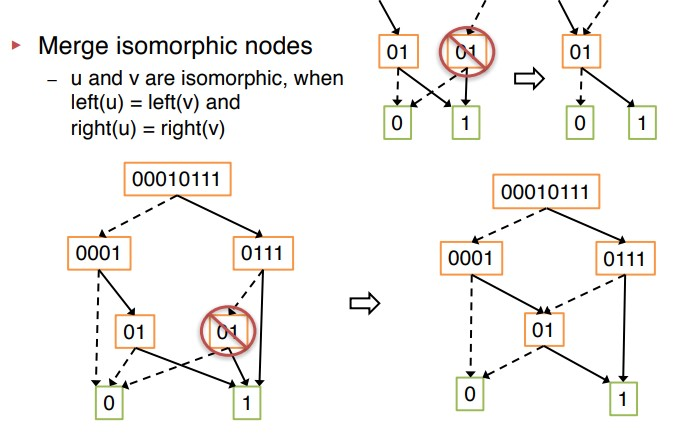
\includegraphics[width=0.8\linewidth]{fig/bdd_reduction3.jpg}
	\end{figure}
\end{itemize}
\begin{figure}[H]
\centering
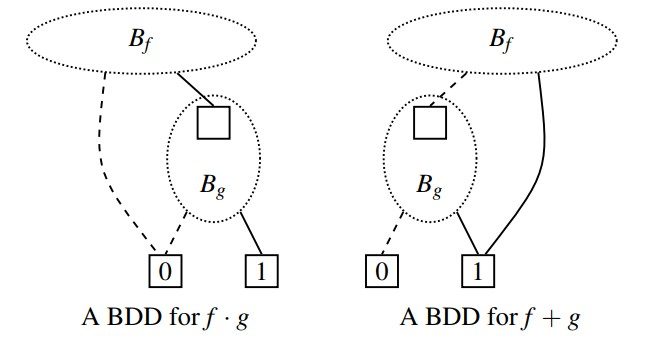
\includegraphics[width=0.6\linewidth]{fig/shortcut_bdd.jpg}
\end{figure}

\begin{definition}[有序BDD]
令$[x_1,\ldots,x_n]$为有序$n$个变量,$B$为含有这些变量的BDD
\begin{itemize}
	\item 令$V(B)$为OBDD的变量集,即$V(B)=\{x_1,x_2,\ldots,x_n\}$
	\item $O_B(x_i)$是$\forall x_i\in V(B)$的序
	\item $\forall x_i,x_j\in V(B),O_B(x_i)<O_B(x_j)$,$B$中任一路径上$x_j$都在$x_i$后面
\end{itemize}
\end{definition}

不同的序会带来不同的OBDD图,导致效率差异。
\begin{figure}[H]
\centering
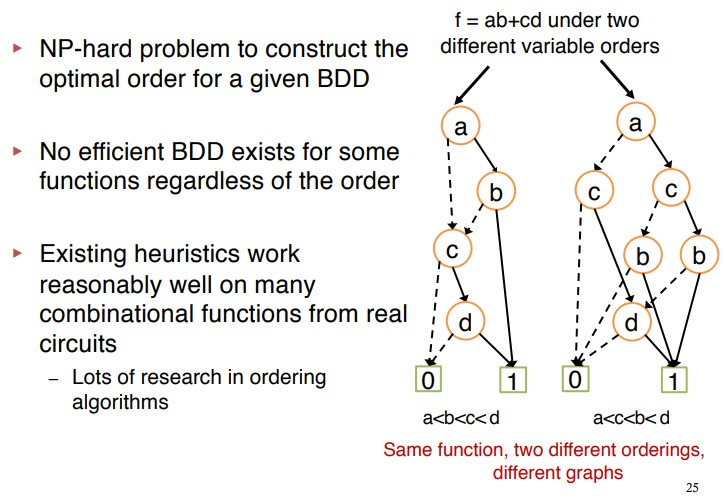
\includegraphics[width=0.8\linewidth]{fig/bdd_limitation.jpg}
\end{figure}

\subsection{约简规则}
\begin{definition}
给定BDD中非终端结点$n$
\begin{itemize}
	\item $lo(n)$是从$n$用虚线指向的点
	\item $hi(n)$是从$n$用实线指向的点
\end{itemize}
$id(\cdot)$为结点编号
\end{definition}

\begin{figure}[H]
\centering
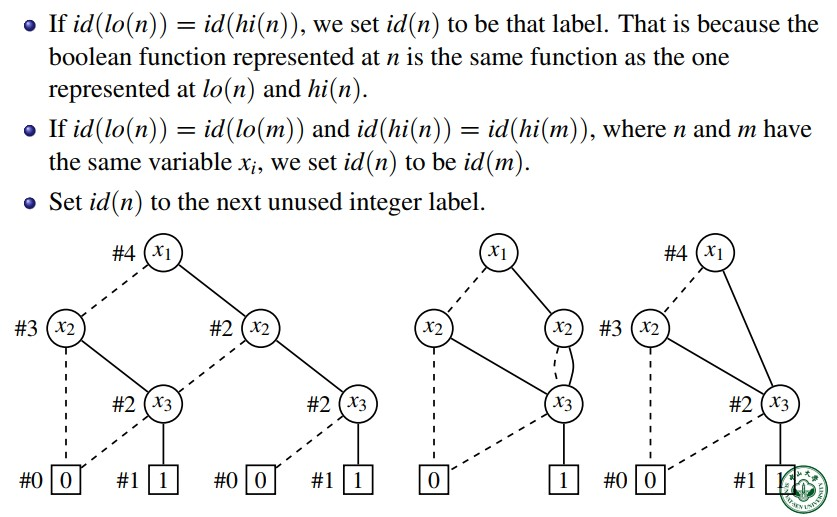
\includegraphics[width=0.8\linewidth]{fig/reduce_alg.jpg}
\end{figure}

约简的BDD图和OBDD可在\href{http://formal.cs.utah.edu:8080/pbl/BDD.php}{这个网页}上在线画图。

\subsection{应用规则}
\begin{definition}[香农展开(Shannon expansion)]
对于所有布尔公式$f$及布尔变量$x$(包括那些不出现在$f$中的),有
\[f\equiv\bar{x}\cdot f[0/x]+x\cdot f[1/x]\]
\end{definition}
应用(apply)函数基于$f \op g$的展开
\[\begin{aligned}
f \op g &\equiv(\bar{x}\cdot f[0/x]+x\cdot f[1/x])\op(\bar{x}\cdot g[0/x]+x\cdot g[1/x])\\
&\equiv(\bar{x}\cdot f[0/x]\op\bar{x}\cdot g[0/x])+(x\cdot f[1/x]\op x\cdot g[1/x])\\
&\equiv\bar{x}\cdot(f[0/x]\op g[0/x])+x\cdot(f[1/x]\op g[1/x])
\end{aligned}\]

\subsection{总结}
\begin{figure}[H]
\centering
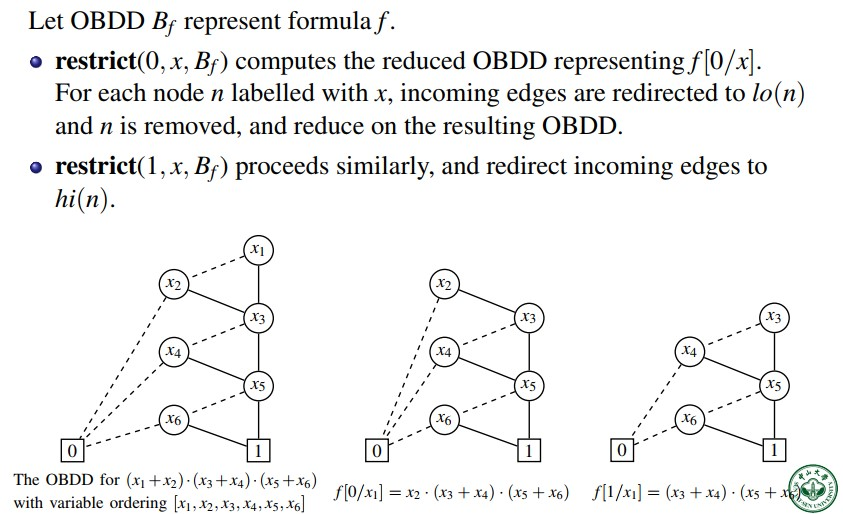
\includegraphics[width=0.8\linewidth]{fig/restrict_alg.jpg}
\end{figure}
\begin{itemize}
\item 特称规则:
\[\exists x.f\eqdef f[0/x]+f[1/x]\]
\item 全称规则:
\[\exists x.f\eqdef f[0/x]\cdot f[1/x]\]
\end{itemize}

\begin{center}
\begin{tabular}{c|l|c|l}
$f$ & OBDD $B_f$ & $f$ & OBDD $B_f$\\\hline
$0$ & $B_0$ & $1$ & $B_1$\\
$x$ & $B_x$ & $\bar{f}$ & 交换$B_f$中的0和1结点\\\hline
$f+g$ & $apply(+,B_f,B_g)$ & $f\cdot g$ & $apply(\cdot,B_f,B_g)$\\
$f\oplus g$ & $apply(\oplus,B_f,B_g)$ & &\\
$f[0/x]$ & $restrict(0,x,B_f)$ & $f[1/x]$ & $restrict(1,x,B_f)$\\\hline
$\exists x.f$ & $apply(+,B_{f[0/x]},B_{f[1/x]})$ & $\forall x.f$ & $apply(\cdot,B_{f[0/x]},B_{f[1/x]})$
\end{tabular}
\end{center}